\documentclass[tikz,border=3pt]{standalone}
\usepackage{fontspec}
\usepackage{amsmath}
\usepackage{xcolor}
\usepackage{tikz}
\usepackage{pgfplots}
\pgfplotsset{compat=1.18}
\usetikzlibrary{arrows.meta,calc,fit,positioning,shapes.geometric,shapes.misc,patterns,plotmarks}
\IfFontExistsTF{Arial}{\setsansfont{Arial}}{\setsansfont{TeX Gyre Heros}}
\renewcommand{\familydefault}{\sfdefault}
\tikzset{
  >={Stealth[length=2.2mm,width=1.5mm]},
  exact title/.style={font=\bfseries\fontsize{10.5}{12}\selectfont,align=center},
  exact subtitle/.style={font=\fontsize{6.3}{7.2}\selectfont,align=center},
  exact label/.style={font=\fontsize{6.4}{7.5}\selectfont,align=center},
  exact tiny/.style={font=\fontsize{5.3}{6.3}\selectfont,align=center},
  panel/.style={draw=black!14,rounded corners=1.2mm,fill=white,line width=.45pt},
  neutral/.style={draw=black!30,fill=black!3,rounded corners=1mm,line width=.45pt},
  arrow/.style={-Stealth,line width=.7pt},
  softarrow/.style={-Stealth,line width=.55pt,draw=black!45},
  dashedarrow/.style={-Stealth,dashed,line width=.55pt,draw=black!55},
  metric/.style={font=\fontsize{5.3}{6.3}\selectfont,fill=white,inner sep=1pt},
}
\newcommand{\pill}[4]{\node[draw=#2!70,fill=#2!10,rounded corners=1.5mm,inner xsep=3pt,inner ysep=2pt,exact label,text=#2] (#1) at #3 {#4};}
\newcommand{\frameboxx}[4]{\draw[draw=#2!65,fill=#2!8,rounded corners=.6mm,line width=.5pt] (#1.south west) rectangle (#1.north east);\node[exact tiny,text=#2] at #3 {#4};}
\newcommand{\axislabel}[3]{\node[exact tiny,text=black!60] at (#1) {#2};\node[exact tiny,text=black!60,rotate=90] at (#3) {#2};}

\definecolor{hiveblue}{HTML}{2F80ED}\definecolor{hivecoral}{HTML}{F28E8E}\definecolor{hivegold}{HTML}{E9C46A}\definecolor{hivegreen}{HTML}{5CB85C}\definecolor{hivepurple}{HTML}{9B7EDE}\definecolor{hiveteal}{HTML}{2A9D8F}\definecolor{hiveink}{HTML}{263238}
\begin{document}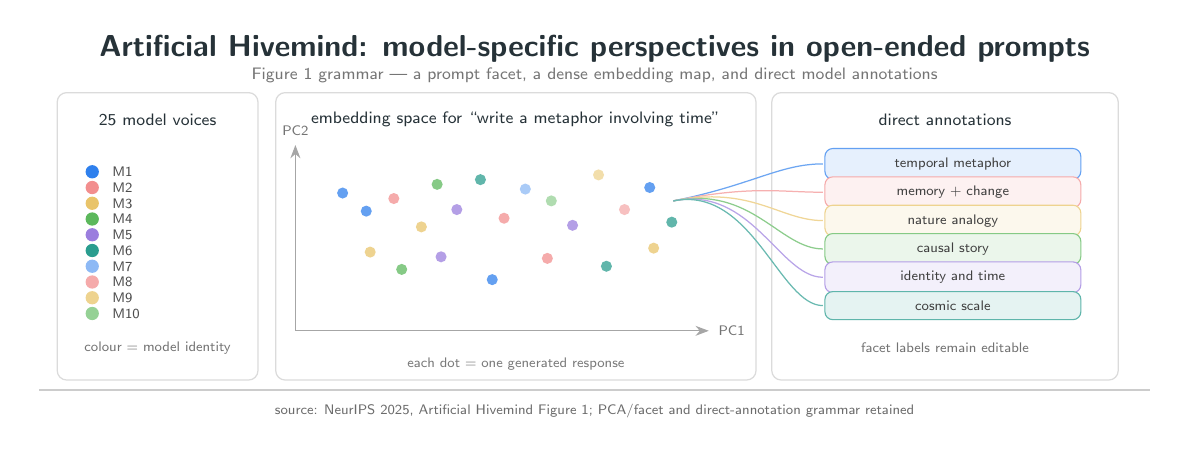
\begin{tikzpicture}[x=1cm,y=1cm]
\path[use as bounding box] (-.2,-2.65) rectangle (14.2,2.65);
\node[exact title,text=hiveink] at (7,2.38) {Artificial Hivemind: model-specific perspectives in open-ended prompts};
\node[exact subtitle,text=black!54] at (7,2.04) {Figure 1 grammar — a prompt facet, a dense embedding map, and direct model annotations};
\node[panel,minimum width=2.55cm,minimum height=3.65cm] (legend) at (1.45,0) {};
\node[exact label,text=hiveink] at (1.45,1.48) {25 model voices};
\foreach \i/\c/\name in {1/hiveblue/M1,2/hivecoral/M2,3/hivegold/M3,4/hivegreen/M4,5/hivepurple/M5,6/hiveteal/M6,7/hiveblue!55/M7,8/hivecoral!75/M8,9/hivegold!75/M9,10/hivegreen!65/M10}{\fill[\c] (.62,1.02-\i*.2) circle (2.4pt);\node[exact tiny,text=black!70,anchor=west] at (.75,1.02-\i*.2) {\name};}
\node[exact tiny,text=black!55] at (1.45,-1.42) {colour = model identity};
\node[panel,minimum width=6.1cm,minimum height=3.65cm] (scatter) at (6.0,0) {};
\node[exact label,text=hiveink] at (6,1.48) {embedding space for “write a metaphor involving time”};
\draw[black!35,-Stealth] (3.2,-1.2) -- (8.45,-1.2) node[right,exact tiny,text=black!55] {PC1};\draw[black!35,-Stealth] (3.2,-1.2) -- (3.2,1.16) node[above,exact tiny,text=black!55] {PC2};
\foreach \x/\y/\c in {3.8/.55/hiveblue,4.1/.32/hiveblue,4.45/.48/hivecoral,4.8/.12/hivegold,5.0/.66/hivegreen,5.25/.34/hivepurple,5.55/.72/hiveteal,5.85/.23/hivecoral,6.12/.6/hiveblue!55,6.45/.45/hivegreen!65,6.72/.14/hivepurple,7.05/.78/hivegold!75,7.38/.34/hivecoral!75,7.7/.62/hiveblue,7.98/.18/hiveteal,4.15/-.2/hivegold,4.55/-.42/hivegreen,5.05/-.26/hivepurple,5.7/-.55/hiveblue,6.4/-.28/hivecoral,7.15/-.38/hiveteal,7.75/-.15/hivegold}{\fill[\c,opacity=.74] (\x,\y) circle (2pt);}
\node[exact tiny,text=black!52] at (6,-1.62) {each dot = one generated response};
\node[panel,minimum width=4.4cm,minimum height=3.65cm] (notes) at (11.45,0) {};
\node[exact label,text=hiveink] at (11.45,1.48) {direct annotations};
\foreach \y/\c/\txt in {.92/hiveblue/temporal metaphor,.56/hivecoral/memory + change,.2/hivegold/nature analogy,-.16/hivegreen/causal story,-.52/hivepurple/identity and time,-.88/hiveteal/cosmic scale}{\node[draw=\c!75,fill=\c!12,rounded corners=1mm,minimum width=3.25cm,minimum height=.3cm,exact tiny,text=black!75] (n\y) at (11.55,\y) {\txt};\draw[\c!70,line width=.45pt] (8.0,.45) .. controls (9.0,.65) and (9.35,\y) .. (9.9,\y);}
\node[exact tiny,text=black!55] at (11.45,-1.42) {facet labels remain editable};
\draw[black!20,line width=.45pt] (-.05,-1.95) -- (14.05,-1.95);
\node[exact tiny,text=black!58] at (7,-2.22) {source: NeurIPS 2025, Artificial Hivemind Figure 1; PCA/facet and direct-annotation grammar retained};
\end{tikzpicture}\end{document}
